\documentclass[relatorio.tex]{subfiles}
\begin{document}
    
\subsection{\textit{Bezier Patches}} \label{subsec:bezier_p}

Numa fase inicial, houve alguma dificuldade, por parte do grupo,
na compreensão sobre a forma de construção das superfícies 3D, através da utilização
da estratégia de \textit{Catmull-Rom}.
Isto deveu-se, essencialmente, a não se estar a efetuar uma interpolação \textit{bilinear},
nem a construção de triângulos. Apenas de linhas.
Depois de se compreender, de facto, como  deveria ser a implementação,
procedeu-se ao desenvolvimento do código apresentado de seguida.

Neste sentido, após uma análise do material fornecido pela equipa docente foram construídas 3 classes para facilitar a definição dos triângulos das superfícies 3D:
\begin{itemize}
    \item \mintinline{cpp}{class Matrix}
    \item \mintinline{cpp}{class PointMatrix}
    \item \mintinline{cpp}{class BezierTriangles}
\end{itemize}

\subsubsection{Classe Matrix}
Envés de representar as matrizes como apontadores para valores, como foi o caso das aulas práticas,
procurou-se definir um módulo que facilmente representaria uma matriz. 
\begin{code}
    \captionof{listing}{Classe Matrix}
    \label{code:class_matrix}
    \inputminted[firstline=14, lastline=19]{cpp}{../../cartesian/matrix.h}
\end{code}

Deste modo, encontram-se na classe todas as operações relativamente a uma matriz e entre matrizes.
Não obstante a possibilidade de \textbf{transpor} e \textbf{clonar} uma matriz,
foi definida a multiplicação entre a matriz local e outra;
como a matriz local pode encontrar-se antes ou depois,
recorreu-se ao \textbf{polimorfismo} da linguagem para construir os dois métodos 
considerando as possibilidades.
Foram definidos construtores que permitissem a criação através do número de linhas e colunas
e aatravés de um conjunto de matrizes default, cf \ref{code:defmat}.

\begin{code}
    \captionof{listing}{Enum de tipos de matrizes default}
    \label{code:defmat}
    \inputminted[firstline=7, lastline=12]{cpp}{../../cartesian/matrix.h}
\end{code}
\dots como são sempre estáticos facilita o grupo ao usá-los nos cálculos dos pontos de uma curvas.

\subsubsection{Class PointMatrix}
Apesar da \mintinline{cpp}{class Matrix} tratar corretamente de matrizes do tipo $float$,
decidiu-se criar um outro tipo de matrizes, com cálculo particulares:
\textbf{matrizes de pontos}. 
Tendo por base a \mintinline{cpp}{class Point} e as necessidades determinadas no desenvolvimento
da presente fase,
criou-se um conjunto de métodos que permitissem a multiplicação entre
uma matriz de valores e uma matriz de pontos, considerando a multiplicação à esquerda e à direita.

Surgiu a \mintinline{cpp}{Classe PointMatrix}:
\begin{code}
    \captionof{listing}{Matrix}
    \label{code:point_matrix.h}
    \inputminted[firstline=6, lastline=10]{cpp}{../../cartesian/PointMatrix.h}
\end{code}
\dots contêm ainda a possibilidade de transpor e clonar a matriz.

A criação desta classe permitiu a implementação das funcionalidades previstas de uma forma
simplificada e elegante, como se poderá ver ao longo do relatório.

\subsubsection{Class BezierTriangles}
Com classes criadas no âmbito de realizar operações entre matrizes,
procedeu-se à criação de uma última: \mintinline{cpp}{class BezierTriangles}.
A partir dos pontos de controlo de um \textit{patch}, permite calcular o ponto da curva,
de acordo com os vetores \textbf{u} e \textbf{v} resultante dos nível de tesselação.
Neste sentido, foi utilizado o médodo apresentado na figura \ref{fig:bezier_point}.
\begin{figure}
    \centering
    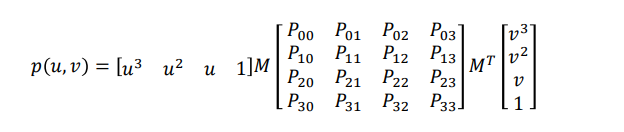
\includegraphics[width=\linewidth]{assets/bezier_patches_point.png}
    \caption{Cálculo de um ponto da superfício, definida com \textit{P} pontos de controlo.}
    \label{fig:bezier_point}
\end{figure}

Assim, segue-se:
\begin{code}
    \captionof{listing}{BezierTriangles}
    \label{code:BezierTriangles.h}
    \inputminted[firstline=5, lastline=15]{cpp}{../../cartesian/BezierTriangles.h}
\end{code}

Para reduzir o número de cálculos a realizar em cada iteração,
considerou-se relevante efetuar um conjunto de pré-calculos que
correspondem à multiplicação da transformação de \textit{Bezier}, $M$, com a matriz dos pontos de controlo da superfície, $P$,
e, consequentemente, o cálculo da resultante, $MxP$, pela transposta de $M$, $M^T$.

\subsubsection{\textit{create\_bezier}}
No âmbito de calcular todas as superfícies criou-se, no módulo \textbf{shapes}, 
um método capaz de contruir um objeto, recebendo um vetor com os índices dos pontos de controlo
de cada \textit{patch}, \textit{pacthes},
um vetor com todos os pontos, \textit{points} e o nível de tesselação, \textit{level},
cf. \ref{code:create_bezier}.

\begin{code}
    \captionof{listing}{create\_bezier}
    \label{code:create_bezier}
    \inputminted[firstline=44, lastline=44]{cpp}{../../generator/shapes.h}
\end{code}

\subsubsection{Adicional}

A extração de informação encontra-se dentro do módulo \textbf{writer}, na função \textit{main} do \textit{generator},
tendo-se utilizado \textbf{expressões regulares}, através da biblioteca \mintinline{cpp}{<regex>}.
Em particular, utiliza-se a expressão \ref{code:regex_pontos}.
\begin{code}
\captionof{listing}{Regex para captura de pontos, utilizando grupos}
\label{code:regex_pontos}
\mintinline{cpp}{regex regexp(R"(([+-]?\d+(?:\.\d+)?), ([+-]?\d+(?:\.\d+)?), ([+-]?\d+(?:\.\d+)?))");}
\end{code}


\end{document}